\chapter{Interface Gráfica (UI)}

\section{Android}
\subsection{Activities}
A plataforma Android oferece algumas opções de criação de interfaces telas. A principal maneira de 
fazê-lo é utilizando uma classe nativa chamada Activity. A classe Activity é responsável por carregar uma 
user interface (UI) é definida através de um arquivo XML de layout usualmente guardado no diretório 
/res/layout do projeto.

No exemplo a seguir, modificado do projeto RestauranteUniversitário, a classe MainActivity herda da classe
AppCompactActivity (um dos tipos de Activity fornecidas pelo Android), e carrega a user interface 
activity\_main.


\lstset{language=Java}

\begin{lstlisting}
// MainActivity.java

package br.ufrj.ct.restauranteuniversitario;

import android.os.Bundle;
import android.support.v7.app.AppCompatActivity;

public class MainActivity extends AppCompatActivity {
    
    @Override
    protected void onCreate(Bundle savedInstanceState) {
        super.onCreate(savedInstanceState);

        //set the layout from the res/layout folder
        setContentView(R.layout.activity_main);
        
     }
}

\end{lstlisting}

Note que o método onCreate é chamado quando a Activity é criada. Ainda mais, existe 
todo um ciclo de vida que define o comportamento de uma Activity dada a interação dela com o 
usuário, conforme mostrado na figura a seguir.

\begin{figure}[htb]
    \centering
    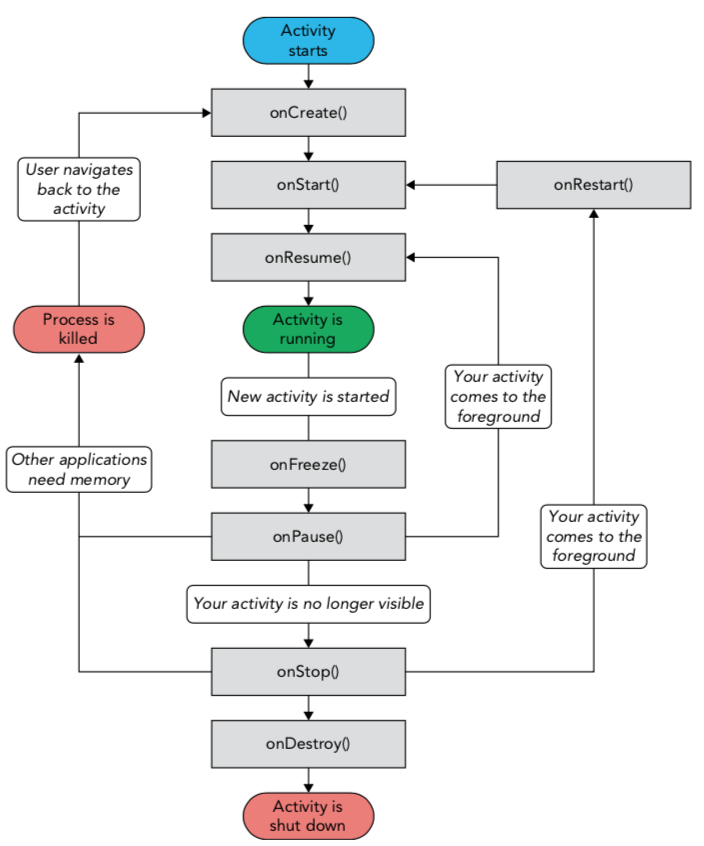
\includegraphics[width=\textwidth]{images/android_activity_lifecycle}
    \caption[Ciclo de vida de uma Activity do Android]
    {Ciclo de vida de uma Activity do Android}%
    \label{fig:android_activity_lifecycle}
\end{figure}


